\section{Proposed method}
A genetic algorithm is a utilization of a population-based strategy for optimization problem, in which each individual is a representation for an acceptable solution. Finding a better solution is a reflection of Darwinian natural selection theory. A more environmentally adaptable individual is, a more survival proportion it has after each generation of evolution.

The mainframe of the genetic algorithm will be described below with a mapping one-to-one with revolutionary theory and a purpose of each component.

\begin{algorithm}
\caption{Genetic algorithm}
\begin{algorithmic}[0]
\State \textbf{Step 1} Initialize population
\State \textbf{Step 2} Evaluation loop
	\While {Stopping conditions are not met}
		\State Crossover
		\State Mutation
		\State Selection
	\EndWhile
\end{algorithmic}
\end{algorithm}

Initialize population is the first and foremost of GA component, which can be considered as our original community. A domain knowledge-based initialize strategy can lead to a huge reduction of computational time. Nevertheless, with a risk of struggling on local search, we highlight generalize characteristics of the population for desiring of cover as much as possible search space. Initialize phase also contains encoding routine, which can be a key in indifference while comparing multiple evolutionary algorithms. This step will be explained in more detail in the following section.

Stopping conditions will be set at the time the population is created. Some most often choices are the maximum number of generations that an individual can reach, the running time of the overall algorithm or the moment when the global fitness value does not change significantly after one generation, in other words, our population is now converged.

A crossover is the main process for creating individuals in the next generation with the intention of keeping good characteristics from older individuals. One can easily see crossover like giving birth to a child hopefully, he will inherit the dominant traits from his parent. And with the help of mutation, when a structure of individual will be fixed in a random way, we can lower the likelihood of falling in local search and even explore a completely new region.

Last but not least, a selection routine can vary from multiple plans, but the final goal is always concentrating on a solution with better fitness value. Yet not defined, a fitness value can be obtained from a fitness function which is a map from an individual representation into a scalar value. A higher fitness value is the metric for the fitness of one individual in the environment, and fitter individuals should live longer than others.

\subsection{Overview}
The first phase of one evolutionary algorithm will be the encoding scheme. Focusing on the solving tree-based problem, numerous encoding strategies were proposed, such as Prufer number, Network Random Keys, Double Layer Encoding. With a high overhead of transforming backward and forward between an individual representation and a Steiner tree for guarantee of feasible characteristics and performing an evolutionary algorithm, we propose using Edge Set as a direct way to encode a solution. The overview of the algorithm is described in the following pseudo-code.

\begin{algorithm}
\caption{GA for MOSTP}
\begin{algorithmic}[0]
\State \textbf{Input} : A graph
\State \textbf{Output}: An individual with minimum fitness value
\State \textbf{Step 1)} Initialization
	\For {Each individual}
		\State \textbf{Step 1.1)} Applying Kruskal for a shuffle edge set of graph to create a tree
		\State \textbf{Step 1.2)} Applying repair scheme to get a Steiner Tree
	\EndFor
\State \textbf{Step 2)} Evaluation loop
	\While {Stopping conditions are not met}
		\State \textbf{Step 2.1)} Using crossover algorithm to create population'
		\State \textbf{Step 2.2)} Using mutation algorithm to create population''
		\State \textbf{Step 2.3)} Using selection routine to get a new population from old population + population' + population''
	\EndWhile
\end{algorithmic}
\end{algorithm}

\subsection{Representation of individual}
No matter how one Steiner tree problem is encoded, two main properties must be held: a sink node and every sensor nodes will be contained and all leaves will be sensor nodes. To achieve a feasible solution, each individual of the population is encoded as a set of edges contained in the tree.

\noindent\makebox[\textwidth]{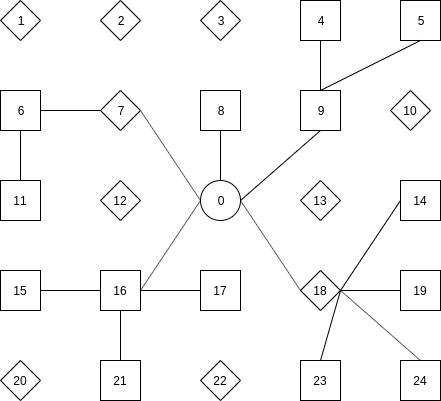
\includegraphics[width=.5\paperwidth]{Images/EdgeSetRepresentation}}

An edge set representation of this tree is: \{(0,7), (0,8), (0,9), (0,16), (7,6), (6,11), (9,4), (9,5), (16,15), (16, 17), (16,21), (18,14), (18,19), (18,23), (18,24)\}.

An Edge-Set representation can be implemented in an array or dictionary with key and values equal to one parent node and its child in the tree. The latter data structure helps reducing fitness value computation as each layer’s structure must be known beforehand to calculate the energy for packet transceiving. It also allows insertion, deletion or lookup of individual edges in constant time, and requires space that is linear with the number of nodes.

This encoding’s natural essence covers some of the most important desirable characteristics of one encoding scheme, which are coverage, unbiasedness, and time. Every tree can be encoded as one edge set and one edge set can only be decoded into one tree. And because we use this representation directly for calculating fitness value and applying evolutionary operators, we can achieve zero-overhead in converting forward and backward between individual and solution. Moreover, its heritability will be maintained with our Kruskal based crossover routine when all common edges between parents will appear in offspring.

Creating a tree by Kruskal algorithm needs a set of edges at first, which is our set of all tuple nodes that have distance smaller than transceiving range. But instead of sorting all edges based on its length, we shuffle the set to get a more generalize population and provide each permutation for Kruskal to construct a tree. We can stop adding an edge to tree when all Steiner nodes were visited and then apply a trimming routine, which will be explained in detail later, to get an attainable solution.

\subsection{Evolutionary operators}
For serving better inheritance methodology, a Kruskal based routine will be applied with a preprocessing of inputted edges.

\begin{algorithm}
\caption{Crossover}
\begin{algorithmic}[0]
\State \textbf{Step 1} Finding intersection between tree 1 and tree 2
\State \textbf{Step 2} Finding disjunctive union between tree 1 and tree 2
\State \textbf{Step 3} Sort disjunctive union based on distance between 2 nodes
\State \textbf{Step 4} Combine 2 groups above and feed for Kruskal to create an offspring
\end{algorithmic}
\end{algorithm}

First of all, we collect all edges appear in both trees, which we hypothesize as a dominant trait that should be inherited by their children. The next step is gathering edges that appear in only tree 1 or tree 2. By containing different attributes for each tree, those edges hold information that enrich different objective. With our own observation that an optimal solution will share some similar properties with a MST, a heuristic scheme can be applied here, which is sorting this disjunctive union by distance from 2 nodes in an edge, then combining with intersection group to form a candidates set for Kruskal algorithm.

\noindent\makebox[\textwidth]{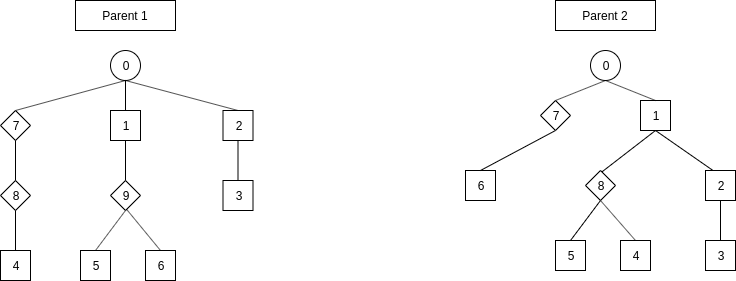
\includegraphics[width=.8\paperwidth]{Images/EdgeSetCrossover}}

The intersection set of these 2 parents is \{(0,1), (0,7), (2,3), (8,4)\} and the disjunctive union set is \{(0,2), (7,8), (1,9), (9,5), (9,6), (7,6), (1,8), (1,2), (8,5)\}. Assume that the sorted version will be the same, we will have a combined group of edges in exact order with these 2 sets. Based on the characteristic of Kruskal algorithm, all edges in the intersection will appear in offspring, then edge in the sorted disjunctive union set will be added if a cycle is not formed.

Calculating each group needs no more than O(m), where m is the length of the longer edge set if we use a dictionary to store information in a tree. And Kruskal algorithm will have amortized time is O((m+n) log (m+1))

This scheme can lead to an unfeasible solution when leaves are not all Steiner nodes, therefore we utilize the repair routine \cite{lu2014construction}. The repair routine is visiting all leaves in the tree and cutting off any leaf which is not a Steiner node. And because after node’s children were cut off tree, it can become unacceptable, leaves trimming strategy is applied until all leaves are satisfactory.

Getting all leaves and removing one can be done in constant time if we construct a set to store all leaves in building tree procedure and a dictionary to get one node’s parent. This repair scheme will acquire at most O(l), where l is the length of the leaves set.

With mutation, we propose a strategy for better generalization of the population.

\begin{algorithm}
\caption{Mutation}
\begin{algorithmic}[0]
\State \textbf{Step 1} Selecting randomly 2 nodes in tree with its distance is smaller than transmission range
\State \textbf{Step 2} Create an edge between 2 nodes
\State \textbf{Step 3} Remove edge from descendant with its older parent
\end{algorithmic}
\end{algorithm}

Reminding that adding another edge between 2 nodes in a tree will definitely lead to an inadmissible when descendant node has 2 parent. A simple proposed solution is removing an older edge between the descendant and its older parent.

\noindent\makebox[\textwidth]{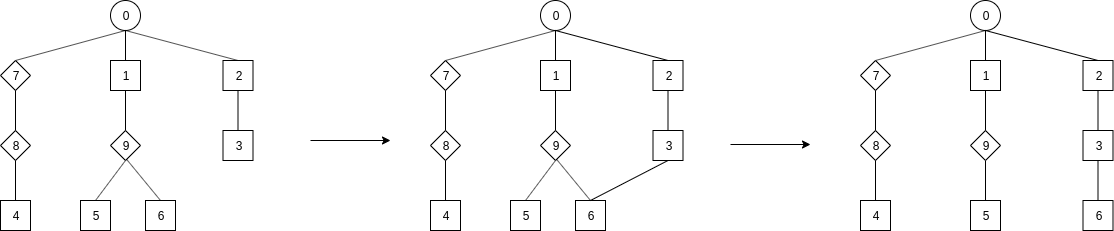
\includegraphics[width=.8\paperwidth]{Images/EdgeSetMutation}} 

The next generation will be chosen by the best selection method, which is only individuals with the best fitness value will be kept. This step takes no more than O(s), where s is the size of the population.